\chapter{Progettazione Concettuale}
\section{Entità e Relazioni}
La seguente tabella riporta una lista completa di tutte le entità e di tutte le relazioni presenti nello schema finale, riportato nella sezione \ref{sec:finalscheme}, in ordine alfabetico.
Per ognuna, viene riportata anche una breve descrizione.\newline
{\rowcolors{3}{black!20!white!50}{black!10!white!50}
\begin{longtable}{ |p{4cm}|p{1.8cm}|p{5.7cm}|  }
%\hline
\endfoot
\hline
\textbf{NOME} & \textbf{TIPO} & \textbf{BREVE DESCRIZIONE} \\
\hline
Aspetto & Entità & Angolazione in gradi\newline tra due Punti del Cielo\\
CasaCoinvolta & Relazione & Lega una specifica casa ad un Placement \\
Casa Astrologica & Entità & Aree sopra e sotto la terra in cui può posizionarsi un Punto del Cielo \\
Domicilio & Relazione & Legame tra i pianeti e i loro segni affini \\
Elemento & Entità & È l'Elemento naturale posseduto da un Segno Zodiacale\\
Essenza & Relazione & Lega gli Elementi ai Segni Zodiacali \\
Governante & Relazione & Lega ogni casa al Segno Zodiacale che la governa\\
Legame & Relazione & L'aspetto che lega due Punti del Cielo di una persona\\
Modalità & Relazione & Lega i modi ai Segni Zodiacali \\
Modo & Entità & È il Modo posseduto da un Segno Zodiacale \\
Orizzonte e Meridiano & Entità & Rappresenta gli estremi dell'orizzonte e del Cielo \\
Persona & Entità & Rappresenta una persona fisica \\
\hline
PersonaAspetto & Relazione & Lega le persone a tutti i suoi aspetti  \\
PersonaCoinvolta & Relazione & Lega le persone a tutti i suoi Placement \\
Pianeta & Entità & Rappresenta un pianeta, più Sole, Luna e Plutone \\
PrimoPuntoAspetto & Relazione & Il primo pianeta legato da un aspetto \\
PuntoCoinvolto & Relazione & L'oggetto coinvolto in un Placement \\
Punto del Cielo & Entità & Supertype di Pianeta, Punto Importante, e Orizz. e Merid. \\
Punto Importante & Entità & Oggetti astratti o corpi fisici non definiti come Pianeti \\
SegnoCoinvolto & Relazione & Il segno coinvolto in un Placement \\
SecondoPuntoAspetto & Relazione & Il secondo pianeta legato da un aspetto \\
Segno Zodiacale & Entità & Rappresenta ogni Segno Zodiacale \\
Tabella degli Aspetti & Entità & Contiene tutti gli Aspetti inseriti\\
Tabella dei Placement & Entità & Contiene tutti i Placement inseriti \\
\hline
\end{longtable}
}
\newpage

\section{Sviluppo di Segni, Modi, Elementi}
La modellazione dei tre concetti, segno, modo, elemento è relativamente semplice da sviluppare.\newline
Segno, modo ed elemento sono entità. Dato che ogni segno ha sia un modo che un elemento, ma lo stesso modo/elemento può comparire in più segni, avremo due relazioni dello stesso tipo.
\begin{figure}[H]
\centering
\includegraphics[width=\textwidth, height=0.35\textheight, keepaspectratio]{img/signmoodelement.png}
\caption{Modellazione di segni, modi ed elementi.}
\label{fig:signmoodelement}
\end{figure}
\textbf{Osservazione:} le tre entità hanno un volume dei dati molto piccolo, ricordiamo che ci sono solo 12 segni, solo 3 modi e solo 4 elementi. Si è preferito comunque separare i tre concetti perchè, in caso contrario, ci sarebbero state ripetizioni nella tabella finale. Inoltre, ogni modo ed ogni elemento hanno un significato astrologico unico, e la descrizione di ognuno deve essere legata agli elementi e ai modi stessi, e non ai segni.

\newpage

\section{Sviluppo di Pianeti e altri Punti}
È importante notare che i pianeti e tutti gli altri corpi (fisici o simbolici che siano) sono due concetti diversi, ma che si comportano sostanzialmente nello stesso modo. Entrambi possono essere legati sia ad una casa che ad un segno, entrambi hanno un nome ed una loro descrizione. È stata scelta una rappresentazione gerarchica per lo schema concettuale finale.
\begin{figure}[H]
\centering
\includegraphics[width=\textwidth, height=0.35\textheight, keepaspectratio]{img/points.png}
\caption{Modellazione di segni, modi ed elementi.}
\label{fig:points}
\end{figure}
Oltre alle due entità Pianeta e Punto Importante, sono stati aggiunti gli estremi dell'orizzonte e il punto più basso e più alto del cielo (Capitolo \ref{cap:int} per i dettagli) sotto il nome dell'entità "Orizzonte e Meridiano". Anche questi ultimi quattro punti si comportano come le altre due subtypes, con la differenza che le case a cui essi sono legati sono statiche, cioè sono le stesse sempre. Il nome della supertype scelto è "Punto del Cielo". La gerarchia è di tipo totale-esclusiva.

\newpage

\section{Sviluppo delle Case}
Le case sono univocamente determinate dal Segno Zodiacale che le governa, per cui, è necessaria un'associazione, denominata "Governante", di cardinalità 1-1 da entrambi i lati. Il software usato per la rappresentazione (Immagine \ref{fig:house}), DB-Main, non permette di rappresentare graficamente l'importazione di una chiave esterna usata come primaria con una relazione di questo tipo. Al momento della traduzione dell’associazione però, la chiave viene correttamente esportata e usata come Identificatore. È stato quindi inserito un post-it per chiarificare questo punto.
\begin{figure}[H]
\centering
\includegraphics[width=\textwidth, height=0.35\textheight, keepaspectratio]{img/house.png}
\caption{Modellazione delle case.}
\label{fig:house}
\end{figure}

\section{Sviluppo del Domicilio}
Il domicilio, funziona in modo simile ai governanti delle case, ma un Pianeta può essere legato a più Segni, ed un Segno può essere domiciliato da più Pianeti. Scorpione per esempio, ha domicilio sia in Marte che in Plutone.\newline
La relazione Domicilio deve quindi legare Pianeta a Segno Zodiacale, e deve avere cardinalità N-M.
\begin{figure}[H]
\centering
\includegraphics[width=\textwidth, height=0.35\textheight, keepaspectratio]{img/domic.png}
\caption{Modellazione della relazione Domicilio.}
\label{fig:domicile}
\end{figure}

\newpage

\section{Persone, Tabella degli Aspetti, Tabella dei Placement}
Ogni persona possiede un Tema Natale. Un Tema Natale contiene al più K Placement, con
\begin{math}
K \equiv |PUNTO \quad DEL \quad CIELO|\end{math}.
Un'entità "Tema Natale" sarebbe stata possibile da inserire, ma non si è scelta questa strada per la creazione del sistema.\newline
L'identificativo della persona fisica, sarebbe di per sè anche lo stesso del Tema Natale. Due persone possono avere lo stesso Tema Natale in sole due condizioni:
\begin{itemize}
  \item Le due persone sono nate a millenni di millenni di anni di distanza tra loro.
  \item Le due persone sono nate lo stesso giorno, alla stessa ora, nello stesso ospedale.
\end{itemize}
Si è quindi scelto di usare una singola entità che contiene tutti i Placement di tutte le Persone. L'identificatore è dato dalla Persona e dal Punto del Cielo coinvolto.\newline
Sarebbe anche stato possibile:
\begin{itemize}
  \item Salvare tutte le possibili coppie di tipo (Punto del Cielo, Casa) e (Punto del Cielo, Segno) in due nuove entità: le tuple dell'entità "Tabella dei Placement" avrebbe avuto un record in meno, al prezzo di inserire altrove circa 300 tuple anticipatamente.
  \item Salvare le oltre 2000 possibili triplette di tipo (Punto del Cielo, Casa, Segno) in una nuova entità: le tuple dell'entità "Tabella dei Placement" avrebbero avuto due record in meno.
\end{itemize}
Le tuple dell'entità "Tabella dei Placement" sono comunque abbastanza piccole, e le ripetizioni delle terne (Punto del Cielo, Casa, Segno) sono poche anche con molti inserimenti.
Per questo è stata scelta la soluzione in figura \ref{fig:placements}.\newline
Come si può notare le tuple finali saranno del tipo:\newline
\textit{(IDPersona, PuntoCoinvolto, SegnoCoinvolto, CasaCoinvolta, Retrogrado)}.\newline
I vincoli sulla retrogradazione dovranno essere gestiti attraverso l'applicativo finale.\newline

\begin{figure}[H]
\centering
\includegraphics[width=\textwidth, height=0.35\textheight, keepaspectratio]{img/placement.png}
\caption{Modellazione della Tabella dei Placement.}
\label{fig:placements}
\end{figure}

La memorizzazione degli aspetti funziona ed è stata pensata essattamente nello stesso modo. Un'entità a parte, denominata "Tabella degli Aspetti" mantiene tutti gli aspetti di tutte le Persone del sistema informatico.\newline
L'identificazione è data dalla persona coinvolta e da entrambi i corpi presi in considerazione nell'aspetto.\newline
Le tuple finali saranno del tipo:\newline
\textit{(IDPersona, Punto1, Aspetto, Punto2)}.

\begin{figure}[H]
\centering
\includegraphics[width=\textwidth, height=0.35\textheight, keepaspectratio]{img/aspects.png}
\caption{Modellazione della Tabella degli aspetti.}
\label{fig:aspects}
\end{figure}

\section{Anteprima dello Schema Finale}
\label{sec:finalscheme}
La prossima pagina contiene la rappresentazione dello schema concettuale finale.\newline
Sono state aggiunte le cardinalità su alcuni attributi.

\newpage

\begin{sidewaysfigure}
  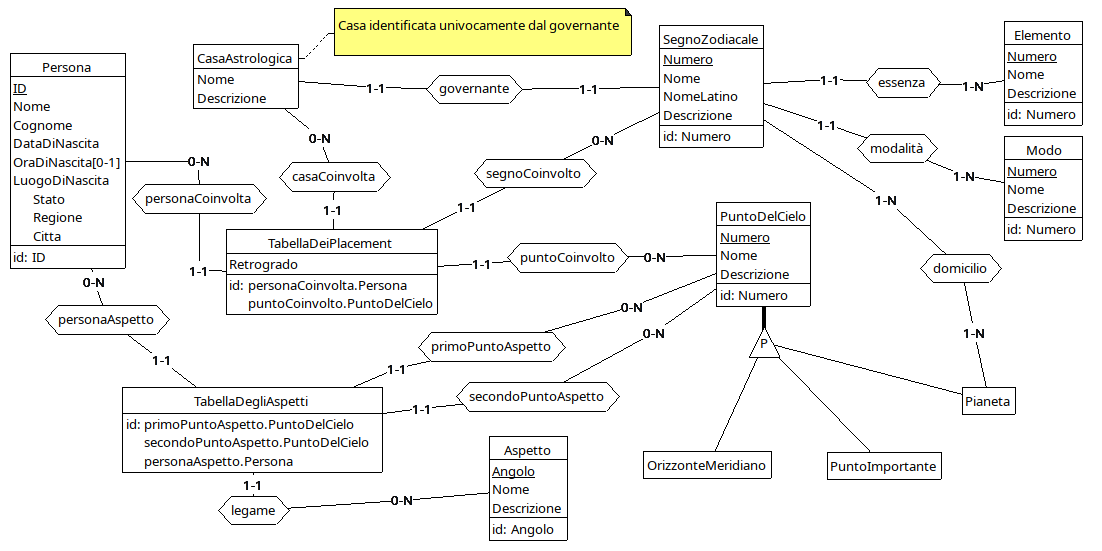
\includegraphics[width=\textwidth,height=\textheight,keepaspectratio]{img/finalscheme.png}
  \caption{Schema concettuale finale}
  \label{fig:finalscheme}
\end{sidewaysfigure}

%
